\section{Experimental Data}
\label{sec:data}

\subsection{Training dataset}
The training data come from two tables of the Supporting Information of Laakso et al.\cite{laakso2025machine} (\path{data/raw/rawdata.xlsx}), whose experimental data were compiled by Song et al.\cite{song2020prediction} (10,116 points for 124 ILs). Table S6 is that compilation, with pressure in bar together with fugacities and UNIFAC activity coefficients; Table S5 is the 1,889-point test set of Laakso et al., taken from the same compilation after removal of duplicates and given with pressure in kPa. Only $T$, $P$ and the \co{} mole fraction $\xco$ were kept. Pressures were converted to kPa and the two tables were concatenated into 12,005 points (\path{notebooks/thesis/02-data-preprocessing.ipynb}). Because Table S5 is a subset of Table S6, and Table S6 itself contains repeated points, the result contains duplicates (Section~\ref{sec:issues}).

Each IL is identified by a cation and an anion abbreviation. The abbreviations were mapped to full ion names (84 unique ions). After merging with the DFT descriptors (Section~\ref{sec:comp}), points whose ions had no successful calculation were dropped. This left the thesis training set of 11,256 points (\path{data/thesis/final_model_dataset_v3.csv}), of which 2,013 are exact repeats of an earlier row (9,243 distinct points). Neither source table gives a reference for each point. Matching against the referenced dataset below traces 8,778 of the 11,256 points (78\%) to one of 106 publications (\path{data/thesis/thesis_point_references.csv}). It is summarised in Table~\ref{tab:dataset} and Fig.~\ref{fig:dataset}; it is dominated by imidazolium cations, and the number of points per IL is uneven, from 1 to 871.

\begin{table}[t]
\caption{The thesis training set (used for the random-split comparison in Table~\ref{tab:metrics}) and the referenced dataset (used for the grouped-validation results in Table~\ref{tab:grouped}).}
\label{tab:dataset}
\centering
\begin{tabular}{lcc}
\toprule
 & \textbf{Thesis set (v3)} & \textbf{Referenced set} \\
\midrule
Data points & 11,256 & 12,297 \\
Ionic liquids & 113 & 109 \\
Cations / anions & 50 / 26 & 39 / 22 \\
Temperature (K) & 243.2--453.2 & 228.2--450.5 \\
Pressure & 0.8~kPa--50.0~MPa & 0.1~kPa--99.0~MPa \\
$\xco$ & 0.00006--0.952 & 0.000004--0.9999 \\
Points per IL (median) & 52 & 68 \\
Source references & Song et al.\cite{song2020prediction} (78\% traced) & 171 publications, DOIs verified \\
Measurement method per point & no & yes \\
\bottomrule
\end{tabular}
\end{table}

\begin{figure}[t]
\centering
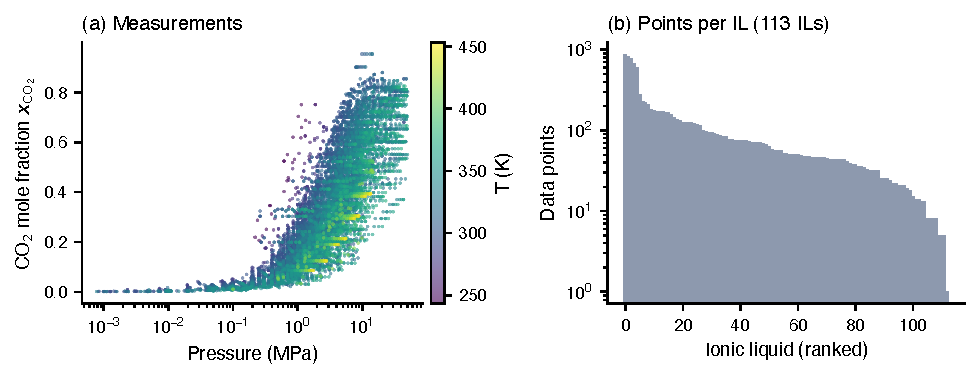
\includegraphics[width=0.9\textwidth]{figures/fig_dataset.pdf}
\caption{Training dataset. (a) \co{} mole fraction against pressure, coloured by temperature. (b) Number of data points for each of the 113 ILs, ranked.}
\label{fig:dataset}
\end{figure}

\subsection{Referenced dataset}
Because the per-point sources were not recorded in the original tables, the dataset was rebuilt from NIST ILThermo\cite{dong2007ilthermo}. The rebuild was restricted to ILs whose cation and anion both have DFT descriptors (\path{scripts/build_referenced_dataset.py}). Molality and mass-fraction data were converted to mole fraction using molar masses computed from the SMILES strings, and exact duplicates were removed. The result has 12,297 points for 109 ILs from 171 publications (2001--2025: 169 journal articles, one book chapter and one PhD thesis). Each point carries the citation, DOI and experimental method. The citations come from ILThermo, but the DOIs were first added from the top hit of a bibliographic search without a check. All 171 were therefore verified against the Crossref record of each publication (title, year, first author and volume; \path{scripts/verify_dataset_references.py}). In 33 publications (2,218 points) the DOI belonged to a different work and in 18 (2,510 points) to a Supporting Information file; 77 points had no DOI. All were corrected, and the outcome of the check for each publication is in \path{data/references/doi_verification.csv}. Static closed-cell measurements make up 35\% of the points and gravimetric methods about 20\%; static closed-cell measurements make up 35\% of the points and gravimetric methods about 20\%. The bibliography is in \path{data/references/dataset_references.bib}. Merged with the corrected descriptors, it gives the model table \path{data/processed/final_referenced_model_dataset_r2scan3c.csv}, which is the basis of the main results (Section~\ref{sec:results}). It is dominated by [Tf$_2$N]$^-$ (4,126 points) and imidazolium cations (82\% of the points).
